% AsymODE on public data: the manuscript with five forecasters on the development tranche of the designed panel
% (DATASET_DESIGN.md v1). Numbers marked \pending{} are filled in when every
% forecaster has five initializations (aris/CYCLE.md, paper phase). Compile on Overleaf (pdflatex).
\documentclass[10pt,twocolumn,letterpaper]{article}
\usepackage[margin=0.75in]{geometry}
\usepackage{amsmath,amssymb,bm}
\usepackage{graphicx,booktabs,xcolor}
\usepackage[hidelinks]{hyperref}
\usepackage{natbib}
\setcitestyle{numbers,square}
\newcommand{\pending}[1]{\textcolor{red}{#1}}
\newcommand{\R}{\mathbb{R}}
% every number of Sections 5-6 comes from these generated files (paper_v1/evaluate_paper.py, counterfactual_v1.py,
% figures_v1.py); a model that is still missing falls back to a red dash
% generated by paper_v1/evaluate_paper.py; do not edit
\newcommand{\SeedsZero}{0}
\newcommand{\RmseZeroOne}{1.128}
\newcommand{\MaeZeroOne}{0.075}
\newcommand{\RmseZeroSix}{1.142}
\newcommand{\MaeZeroSix}{0.076}
\newcommand{\RmseZeroTwentyFour}{1.166}
\newcommand{\MaeZeroTwentyFour}{0.073}
\newcommand{\RmseZeroFortyEight}{1.093}
\newcommand{\MaeZeroFortyEight}{0.064}
\newcommand{\ZeroVsHostOne}{$+$1.6\%}
\newcommand{\ZeroVsHostOneCI}{[$-$0.0, $+$3.1]}
\newcommand{\ZeroVsHostSix}{$+$1.4\%}
\newcommand{\ZeroVsHostSixCI}{[$-$0.1, $+$2.8]}
\newcommand{\ZeroVsHostTwentyFour}{$+$1.7\%}
\newcommand{\ZeroVsHostTwentyFourCI}{[$+$0.4, $+$3.1]}
\newcommand{\ZeroVsHostFortyEight}{$+$1.2\%}
\newcommand{\ZeroVsHostFortyEightCI}{[$+$0.3, $+$2.4]}
\newcommand{\ZeroVsHostTropical}{$+$6.2\%}
\newcommand{\ZeroVsHostWinter}{$+$1.3\%}
\newcommand{\ZeroVsHostSynoptic}{$-$4.1\%}
\newcommand{\ZeroVsHostConvective}{$+$1.5\%}
\newcommand{\ZeroVsHostRain}{$-$3.5\%}
\newcommand{\SeedsHost}{5}
\newcommand{\RmseHostOne}{1.110}
\newcommand{\MaeHostOne}{0.150}
\newcommand{\RmseHostSix}{1.126}
\newcommand{\MaeHostSix}{0.151}
\newcommand{\RmseHostTwentyFour}{1.147}
\newcommand{\MaeHostTwentyFour}{0.144}
\newcommand{\RmseHostFortyEight}{1.080}
\newcommand{\MaeHostFortyEight}{0.126}
\newcommand{\HostVsZeroOne}{$-$1.6\%}
\newcommand{\HostVsZeroOneCI}{[$-$3.0, $+$0.0]}
\newcommand{\HostVsZeroSix}{$-$1.4\%}
\newcommand{\HostVsZeroSixCI}{[$-$2.8, $+$0.1]}
\newcommand{\HostVsZeroTwentyFour}{$-$1.7\%}
\newcommand{\HostVsZeroTwentyFourCI}{[$-$3.0, $-$0.4]}
\newcommand{\HostVsZeroFortyEight}{$-$1.2\%}
\newcommand{\HostVsZeroFortyEightCI}{[$-$2.3, $-$0.3]}
\newcommand{\HostVsZeroTropical}{$-$5.8\%}
\newcommand{\HostVsZeroWinter}{$-$1.3\%}
\newcommand{\HostVsZeroSynoptic}{$+$4.3\%}
\newcommand{\HostVsZeroConvective}{$-$1.5\%}
\newcommand{\HostVsZeroRain}{$+$3.7\%}
\newcommand{\SeedsGCRK}{1}
\newcommand{\RmseGCRKOne}{1.117}
\newcommand{\MaeGCRKOne}{0.141}
\newcommand{\RmseGCRKSix}{1.133}
\newcommand{\MaeGCRKSix}{0.143}
\newcommand{\RmseGCRKTwentyFour}{1.156}
\newcommand{\MaeGCRKTwentyFour}{0.136}
\newcommand{\RmseGCRKFortyEight}{1.087}
\newcommand{\MaeGCRKFortyEight}{0.120}
\newcommand{\GCRKVsHostOne}{$+$0.7\%}
\newcommand{\GCRKVsHostOneCI}{[$-$0.1, $+$1.7]}
\newcommand{\GCRKVsHostSix}{$+$0.7\%}
\newcommand{\GCRKVsHostSixCI}{[$-$0.2, $+$1.7]}
\newcommand{\GCRKVsHostTwentyFour}{$+$0.8\%}
\newcommand{\GCRKVsHostTwentyFourCI}{[$-$0.1, $+$1.9]}
\newcommand{\GCRKVsHostFortyEight}{$+$0.7\%}
\newcommand{\GCRKVsHostFortyEightCI}{[$+$0.1, $+$1.7]}
\newcommand{\GCRKVsHostTropical}{$+$0.2\%}
\newcommand{\GCRKVsHostWinter}{$+$0.9\%}
\newcommand{\GCRKVsHostSynoptic}{$+$1.4\%}
\newcommand{\GCRKVsHostConvective}{$+$0.3\%}
\newcommand{\GCRKVsHostRain}{$+$1.2\%}
\newcommand{\GCRKVsZeroOne}{$-$0.9\%}
\newcommand{\GCRKVsZeroOneCI}{[$-$2.0, $+$0.3]}
\newcommand{\GCRKVsZeroSix}{$-$0.7\%}
\newcommand{\GCRKVsZeroSixCI}{[$-$1.8, $+$0.5]}
\newcommand{\GCRKVsZeroTwentyFour}{$-$0.9\%}
\newcommand{\GCRKVsZeroTwentyFourCI}{[$-$2.0, $+$0.2]}
\newcommand{\GCRKVsZeroFortyEight}{$-$0.5\%}
\newcommand{\GCRKVsZeroFortyEightCI}{[$-$1.3, $+$0.5]}
\newcommand{\GCRKVsZeroTropical}{$-$5.6\%}
\newcommand{\GCRKVsZeroWinter}{$-$0.5\%}
\newcommand{\GCRKVsZeroSynoptic}{$+$5.8\%}
\newcommand{\GCRKVsZeroConvective}{$-$1.1\%}
\newcommand{\GCRKVsZeroRain}{$+$5.0\%}
\newcommand{\GCRKSeedsBetter}{0}
\newcommand{\GCRKSeedRange}{$+$0.4\% to $+$0.4\%}
\newcommand{\ZeroVsHostDropThree}{$+$1.4\%}
\newcommand{\GCRKVsHostDropThree}{$+$0.5\%}
\newcommand{\ZeroVsHostDropFive}{$+$1.7\%}
\newcommand{\GCRKVsHostDropFive}{$+$0.6\%}
\newcommand{\NServed}{8{,}051}
\newcommand{\NStock}{406}
\newcommand{\ZeroVsHostServed}{$+$1.3\%}
\newcommand{\GCRKVsHostServed}{$+$0.7\%}
\newcommand{\ZeroVsHostStock}{$+$5.0\%}
\newcommand{\GCRKVsHostStock}{$+$0.1\%}
\newcommand{\NLarge}{726}
\newcommand{\HostPeakRatio}{8\%}
\newcommand{\HostHalfPeak}{2\%}
\newcommand{\GCRKPeakRatio}{9\%}
\newcommand{\GCRKHalfPeak}{8\%}

% generated by paper_v1/describe_v1.py; do not edit
\newcommand{\NEvents}{8{,}457}
\newcommand{\NCounties}{2{,}410}
\newcommand{\NStates}{42}
\newcommand{\NSystems}{81}
\newcommand{\NRenewed}{2{,}225}
\newcommand{\ShareRenewed}{26\%}
\newcommand{\NServedAtOrigin}{5{,}802}
\newcommand{\NInitiated}{1{,}639}
\newcommand{\ShareRenewedTropical}{37\%}
\newcommand{\ShareRenewedWinter}{21\%}
\newcommand{\ShareRenewedSynoptic}{31\%}
\newcommand{\ShareRenewedConvective}{21\%}
\newcommand{\ShareRenewedRain}{21\%}

% generated by paper_v1/counterfactual_v1.py; do not edit
\newcommand{\CfGCRKAll}{$+$2.5\%}
\newcommand{\CfGCRKTropical}{$+$1.0\%}
\newcommand{\CfGCRKWinter}{$+$5.0\%}
\newcommand{\CfGCRKSynoptic}{$+$1.9\%}
\newcommand{\CfGCRKConvective}{$+$0.1\%}
\newcommand{\CfGCRKRain}{$-$0.9\%}
\newcommand{\CfGCRKDpeak}{0.26}
\newcommand{\CfGCRKMoved}{4\%}
\newcommand{\CfGCRKSeeds}{1}
\newcommand{\CfModAll}{$-$0.8\%}
\newcommand{\CfModTropical}{$-$3.9\%}
\newcommand{\CfModWinter}{$-$1.6\%}
\newcommand{\CfModSynoptic}{$+$8.6\%}
\newcommand{\CfModConvective}{$+$0.0\%}
\newcommand{\CfModRain}{$-$0.7\%}
\newcommand{\CfModDpeak}{0.45}
\newcommand{\CfModMoved}{15\%}
\newcommand{\CfModSeeds}{3}
\newcommand{\CfHazAll}{$-$3.3\%}
\newcommand{\CfHazTropical}{$-$4.5\%}
\newcommand{\CfHazWinter}{$-$6.8\%}
\newcommand{\CfHazSynoptic}{$+$10.0\%}
\newcommand{\CfHazConvective}{$+$0.1\%}
\newcommand{\CfHazRain}{$-$1.1\%}
\newcommand{\CfHazDpeak}{0.67}
\newcommand{\CfHazMoved}{23\%}
\newcommand{\CfHazSeeds}{3}

\IfFileExists{generated/numbers_fig4.tex}{% generated by paper_v1/figures_v1.py; do not edit
\newcommand{\FigFourNameA}{Vernon, LA}
\newcommand{\FigFourObsA}{83\%}
\newcommand{\FigFourHostA}{5\%}
\newcommand{\FigFourGCRKA}{23\%}
\newcommand{\FigFourNameB}{Sabine, LA}
\newcommand{\FigFourObsB}{14\%}
\newcommand{\FigFourHostB}{5\%}
\newcommand{\FigFourGCRKB}{23\%}
\newcommand{\FigFourNameC}{Nantucket, MA}
\newcommand{\FigFourObsC}{83\%}
\newcommand{\FigFourHostC}{5\%}
\newcommand{\FigFourGCRKC}{5\%}
\newcommand{\FigFourNameD}{Dukes, MA}
\newcommand{\FigFourObsD}{8\%}
\newcommand{\FigFourHostD}{5\%}
\newcommand{\FigFourGCRKD}{5\%}
\newcommand{\FigFourNameE}{Yates, NY}
\newcommand{\FigFourObsE}{63\%}
\newcommand{\FigFourHostE}{3\%}
\newcommand{\FigFourGCRKE}{2\%}
\newcommand{\FigFourNameF}{Carter, OK}
\newcommand{\FigFourObsF}{42\%}
\newcommand{\FigFourHostF}{3\%}
\newcommand{\FigFourGCRKF}{3\%}
\newcommand{\FigFourNameG}{Tehama, CA}
\newcommand{\FigFourObsG}{63\%}
\newcommand{\FigFourHostG}{1\%}
\newcommand{\FigFourGCRKG}{1\%}
\newcommand{\FigFourNameH}{East Feliciana, LA}
\newcommand{\FigFourObsH}{97\%}
\newcommand{\FigFourHostH}{5\%}
\newcommand{\FigFourGCRKH}{38\%}
\newcommand{\FigFourMaxEFG}{3\%}
}{}
\providecommand{\TimesFMVsHostOne}{\pending{--}}\providecommand{\TimesFMVsHostOneCI}{\pending{--}}
\providecommand{\TimesFMVsHostFortyEight}{\pending{--}}\providecommand{\TimesFMVsHostFortyEightCI}{\pending{--}}
\providecommand{\TimesFMVsZeroOne}{\pending{--}}\providecommand{\TimesFMVsZeroFortyEight}{\pending{--}}
\providecommand{\TimesFMPeakRatio}{\pending{--}}\providecommand{\TimesFMHalfPeak}{\pending{--}}
\providecommand{\TimesFMVsHostDropThree}{\pending{--}}

\title{Asymmetric Outage Dynamics with Geography and Weather:\\ County-Level Forecasts from Public Data}
\author{\pending{Authors to be confirmed}}
\date{}

\begin{document}
\maketitle

\begin{abstract}
Successive storms can cause new interruptions while earlier outages are still being restored, so an outage forecast
must track both the continuing effect of weather and the customers still without service. We develop AsymODE, a
population-balance forecaster in which damage acts on customers still served and recovery on customers already out,
each with its own neural rate and inputs, and a Geography-Conditioned Response Kernel (GCRK) inside the damage
network that lets terrain, soil and land cover set how a bounded memory of weather fades, interacts and is read out.
We evaluate on public data only: EAGLE-I county outage records, ERA5 weather, and a designed panel of 81 weather
systems of five regimes drawn with known probabilities from 20,830 NWS-warning-defined systems of 2018--2025, with
every system held out in turn. From one open-loop trajectory per county-event, every forecaster stays close to the
all-zero forecast in pooled RMSE: AsymODE's RMSE relative to it is \HostVsZeroOne\ at +1~hour and
\HostVsZeroFortyEight\ at +48~hours, with gains in tropical-cyclone, convective and winter systems and losses in
synoptic windstorms and heavy rain. Relative to AsymODE, zero-shot TimesFM's RMSE is \TimesFMVsHostOne\ and
\TimesFMVsHostFortyEight\ at these horizons, and GCRK's \GCRKVsHostOne\ and \GCRKVsHostFortyEight. Neighbouring
counties with nearly the same weather but very different outages remain unresolved, and the largest outages are
forecast at a small fraction of their size.
\end{abstract}

\section{Introduction}
When a second storm arrives, new interruptions can occur while customers affected by the first are still waiting for
service. A forecast of the number without power must therefore anticipate both the next disruption and the evolution of
the existing outage stock: a high but declining outage level calls for different preparation from a low level about to
rise. Public county outage records now make this problem measurable across the United States and across weather
regimes, from convective lines to tropical cyclones and ice storms~\cite{brelsford2024}.

Two lines of work inform such forecasts. Weather-based outage prediction has established the importance of local
exposure: weather combined with soil, vegetation and utility assets predicts storm outages~\cite{cerrai2019}, tracked
storms and forest characteristics predict damage categories~\cite{tervo2021}, and dynamic prediction exploits evolving
weather sequences~\cite{alpay2020}. Process-based models describe how outages unfold: Dobson~\cite{dobson2023}
connects outage and restoration processes to resilience curves, and Zhu et al.~\cite{zhu2025} place discounted weather
accumulation, a nonlinear weather response and outage-history triggering inside a spatiotemporal model of customer
outages. Together they indicate that the effect of weather outlasts the hour in which it occurs and depends on the
environment it meets.

An open-loop forecast through a later storm raises two design questions. The first is which population each process
acts on. We adopt a population balance in which damage acts on customers still served and recovery on customers
currently out, so the two processes can respond to different information, operate simultaneously, and start an outage
in a fully served county. The second is how fixed geography should enter a response that changes hour by hour.
Supplied as ordinary features, terrain, vegetation and soil descriptors act as county-specific intercepts. GCRK
instead lets a county's geography shape the geometry of a single fading response state~\cite{zhu2021hotspots}, so
that geography changes how a weather sequence is processed rather than what level is predicted.

Our contributions are threefold. (i) A population-balance forecaster whose damage and recovery rates read different
information and act on different source populations. (ii) A Geography-Conditioned Response Kernel in the damage network's hidden
layer, whose explicit, ordered kernel lets geography set how the effects of weather fade, interact and are read out. (iii) A public,
designed benchmark: weather systems of five regimes drawn with recorded inclusion probabilities, observation gates that
never read the forecast window, and an event-held-out evaluation in which every forecast concerns a storm the model
has not seen.

\section{Data and Empirical Motivation}
\subsection{Weather systems drawn from a public frame}
The frame lists every weather system defined by National Weather Service warnings in the contiguous United States
between July 2018 and December 2025, from the Iowa Environmental Mesonet VTEC archive and the NHC best
tracks~\cite{landsea2013}: warnings linked in space and time form a system, tropical warnings join their storm, and each
system is typed as convective, synoptic wind, tropical cyclone, winter or heavy rain. Of 28,229 systems, 20,830 pass
outcome-independent data gates. A development tranche of 81 systems was drawn with probability proportional to the
customers under warnings: 15 per regime, and a registered supplementary draw that added three synoptic-wind systems of
an under-represented season and three heavy-rain systems far from the coast when the geography and season audit of the
first draw failed; a separate tranche of 99 systems is sealed for a later confirmatory test and is not used here. Within each
system, at most 140 counties are drawn, 90 under a warning, 25 under an advisory or watch and 25 from a ring within
200~km that received no product, with probability proportional to a reanalysis hazard index that never enters a model,
so that near misses are represented. The panel holds \NEvents\ county-events in \NCounties\ counties of \NStates\
states. Every metric
and loss carries the design weight $w=1/(\pi_{\text{system}}\,\pi_{\text{county}})$, trimmed at ten times its
regime's median, so that the sample stands for the frame.

Let $p_{i,t}$ denote the fraction of customers without service in county-event $i$ at hour $t=0,\dots,215$, from
EAGLE-I county records divided by the publisher's 2024 modelled customers~\cite{brelsford2024}. The forecast origin is
hour 72, six hours before the first warning's expected onset; outage observations are used through hour 71, and ERA5
weather~\cite{hersbach2020} is supplied for all 216 hours, so every compared forecast is conditioned on the realised
weather. Figure~\ref{fig:impacts} maps the county impacts of the development systems.

\begin{figure*}[t]
\centering
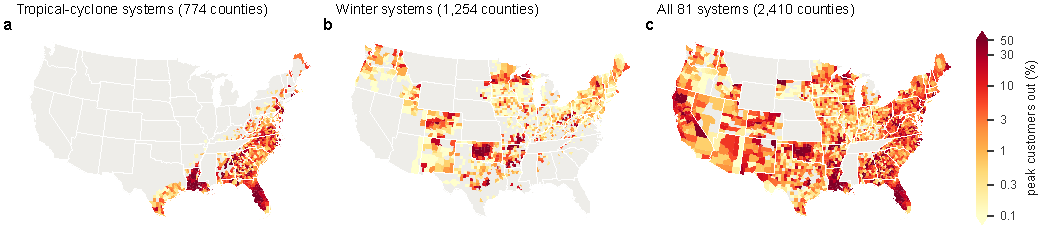
\includegraphics[width=\textwidth]{figures/fig1_impacts_v1.pdf}
\caption{County-level peak outage fractions in the development tranche: (a) tropical-cyclone systems, (b) winter
systems, (c) all 81 systems. A county that appears in several systems shows its largest peak.}
\label{fig:impacts}
\end{figure*}

\subsection{Initiation, renewed growth and geographic context}
\label{sec:context}
County records aggregate concurrent interruption and restoration; their difference determines the change in outage
stock, and the two gross processes are latent. Renewed growth is common: in \NRenewed\ of the \NEvents\ county-events
(\ShareRenewed) the outage fraction rises by at least two percentage points within two hours during the forecast
window, most often in tropical (\ShareRenewedTropical) and synoptic-wind (\ShareRenewedSynoptic) systems;
\NInitiated\ of the \NServedAtOrigin\ county-events with no customers out at hour 71 later reach at least 2\%. Forecasts must therefore support both renewed growth and initiation from a fully served
state.

County differences also motivate a conditional weather response. We call two neighbouring counties of the same
system weather twins when both serve at least 5,000 customers, their hourly reanalysis gusts and precipitation over the
forecast window correlate at no less than 0.95 and 0.90, and their maximum gusts and precipitation totals differ by at
most 10\% and 25\%. The twins with the largest difference in 3-hour peak outage fraction are, among tropical systems,
Vernon and Sabine parishes, Louisiana, in Hurricane Delta (2020): maximum gusts of 22.9 and 22.1~m\,s$^{-1}$ and 127
and 133~mm of precipitation, yet peaks of 83\% and 14\%. Among winter systems they are Nantucket and Dukes counties,
Massachusetts, in the blizzard of late January 2022: gusts of 33.5 and 32.9~m\,s$^{-1}$, correlated at 0.99, and peaks
of 83\% and 8\%.

Geography and weather regime are strongly confounded. Tropical systems land on dense-canopy, flat, poorly drained and
densely served coastal counties (median canopy 49\%, 93~km from the coast); synoptic windstorms land on open, rugged,
well-drained inland counties (16\%, 724~km). A geographic effect can therefore only be learned within regimes, and the
design audits the geography of every regime. We use 40 public county descriptors of terrain (USGS 3DEP), tree canopy and
land cover (USFS NLCD, 2021), soils (SSURGO and gNATSGO), forest land (FIA) and their co-location. Table~\ref{tab:inputs} summarizes which information
reaches which process.

\begin{table}[t]
\centering\small
\caption{Information routes. Outage-derived inputs use hours 0--71 only; county identifiers are not inputs.}
\label{tab:inputs}
\begin{tabular}{@{}p{0.27\columnwidth}p{0.66\columnwidth}@{}}
\toprule
Information & Role\\
\midrule
Local weather & ERA5 channels and causal summaries for damage; selected weather for recovery.\\
Natural geography & 40 descriptors control the GCRK response and its damage-side readout.\\
Observed outages & Prefix summaries inform recovery; $p_{i,71}$ initializes the stock.\\
County context & Customer scale, rural--urban code, population density, utility mix and 2017 reliability (EIA-861), and
the weather of the five nearest counties inform recovery.\\
\bottomrule
\end{tabular}
\end{table}

\subsection{One trajectory, scored along its path}
The prediction target is $p_{i,t}$ itself. From the observed $p_{i,71}$ each model produces one open-loop path over hours
72--215, and every metric is computed on that path. As in forecasts issued at later origins, we score each lead $h$ by
the error of the path at hours $72+h,\dots,215$ and report $h=1,6,24,48$.

\section{Asymmetric Neural Outage Dynamics}
\subsection{Transitions from different source populations}
Let $u_{i,t}$ be the fraction of the previously served population interrupted during hour $t$ and $r_{i,t}$ the fraction of
the previously outaged population restored. The two rates drive the hourly population balance
\begin{equation}
p_{i,t}=p_{i,t-1}+u_{i,t}(1-p_{i,t-1})-r_{i,t}\,p_{i,t-1}, \label{eq:balance}
\end{equation}
the hourly counterpart of $\dot p=\lambda_U(1-p)-\lambda_R p$ with bounded one-step transition
fractions~\cite{chen2018}. Because $p_{i,t}=(1-p_{i,t-1})u_{i,t}+p_{i,t-1}(1-r_{i,t})$ is a convex combination of values in
$[0,1]$, the stock stays valid, and at $p_{i,t-1}=0$ the balance gives $p_{i,t}=u_{i,t}$, so an outage can start in a fully
served county; contagion-only inflow proportional to $p(1-p)$, as in unforced epidemic models~\cite{kermack1927}, would
leave zero absorbing.

\subsection{Process-specific neural mappings}
The damage and recovery networks have independent parameters and inputs, shared across counties within each process.
Damage is a two-hidden-layer MLP of width 32 over the weather inputs, with a learned logit smoother, a weather-based
occurrence gate and a small background rate; recovery is an independent two-hidden-layer MLP of width 16 over selected
weather, the observed prefix and the county context, recomputed at every forecast hour. The asymmetry lies in the
allocation of information, neural structure and source populations. Figure~\ref{fig:model} shows the two rate
networks, the kernel of Section~\ref{sec:routes} inside the damage network and the balance that joins them.

\begin{figure*}[t]
\centering
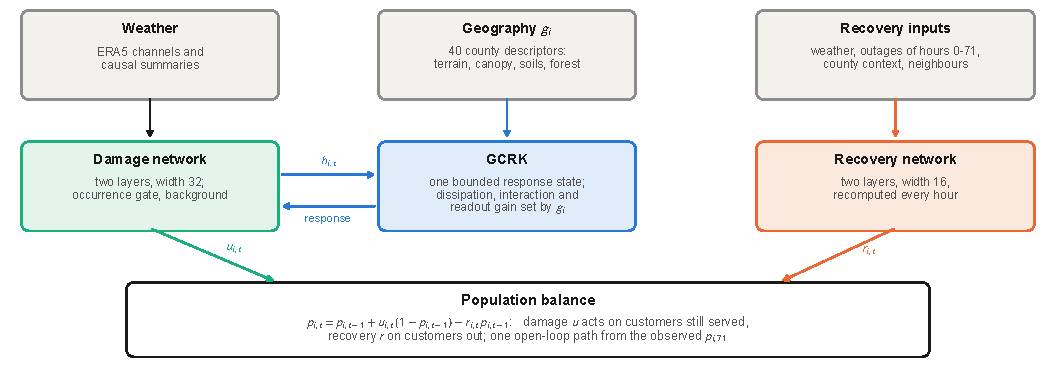
\includegraphics[width=\textwidth]{figures/fig2_model_v1.pdf}
\caption{AsymODE with GCRK. The damage network reads weather; GCRK, inside it, turns the departures of its first
hidden representation $h_{i,t}$ into one bounded response state whose dissipation, interaction and readout gain are
set by the county's descriptors. The recovery network reads selected weather, the observed
prefix and the county context. The population balance applies damage to customers still served and recovery to
customers out.}
\label{fig:model}
\end{figure*}

\section{Geography-Conditioned Response Kernel}
\label{sec:routes}
GCRK sits inside the damage network and advances one bounded response state through a dissipative, input-dependent
operator. Departures of the damage network's hidden representation from its causal prefix reference drive the state; a
four-dimensional code of the county's descriptors sets the dissipation rates, a skew-symmetric interaction direction
and a readout gain, so geography changes how a weather sequence is processed rather than what level is predicted. The
state has an explicit, ordered response kernel and a unit bound, with an $O(d)$ solve per county-hour. The kernel's
opening is bounded (a $\tanh$ of a learned scalar); on this panel, an unbounded opening improved tropical systems but
worsened synoptic wind and heavy rain.

\section{Forecasting Results and Interpretation}
\subsection{Training}
Every learned model minimizes the design-weighted MSE of $p$ over hours 72--215, with each regime normalized by its
all-zero error in the training folds so that no regime dominates. Training uses Adam for 900 steps with paired
initialization: models of the same seed start from the same host parameters, and the kernel's contribution starts at
zero and opens over the first 200 steps, so that at step 0 AsymODE + GCRK equals AsymODE. Five initializations are averaged in forecast space.

\subsection{Event-held-out evaluation}
Whole weather systems are held out: families of linked systems, joined when they share a county within 16 days, form
five folds, balanced by regime. Every county-event is forecast by models that never saw its storm. We include TimesFM, a
decoder-only foundation model for time series~\cite{das2024}, zero-shot from its official checkpoint, with the observed
customers out over hours 0--71 as context and the same 14 weather channels over all 216 hours as covariates.
Table~\ref{tab:accuracy} compares the five forecasters.

\begin{table*}[t]
\centering\small
\caption{Forecast accuracy on the development tranche, every weather system held out (five folds), in percentage
points of customers. Errors of the one open-loop path per county-event are pooled over the held-out county-hours with
the design weights; learned models average five initializations ($^{\dagger k}$: provisional, $k$ of five so far).
Lower is better; the best value in each column is in bold.}
\label{tab:accuracy}
\begin{tabular}{@{}lcccccccc@{}}
\toprule
 & \multicolumn{4}{c}{MAE} & \multicolumn{4}{c}{RMSE}\\
\cmidrule(lr){2-5}\cmidrule(l){6-9}
Model & +1 h & +6 h & +24 h & +48 h & +1 h & +6 h & +24 h & +48 h\\
\midrule
All zero & \textbf{0.075} & \textbf{0.076} & \textbf{0.073} & \textbf{0.064} & 1.128 & 1.142 & 1.166 & 1.093 \\
TimesFM & -- & -- & -- & -- & -- & -- & -- & -- \\
AsymODE & 0.150 & 0.151 & 0.144 & 0.126 & 1.110 & 1.126 & 1.147 & 1.080 \\
AsymODE + GCRK$^{\dagger1}$ & 0.141 & 0.143 & 0.136 & 0.120 & 1.117 & 1.133 & 1.156 & 1.087 \\
AsymODE + geography $\times$ weather$^{\dagger3}$ & 0.156 & 0.158 & 0.150 & 0.132 & \textbf{1.092} & \textbf{1.107} & \textbf{1.124} & \textbf{1.057} \\

\bottomrule
\end{tabular}
\end{table*}

Three features stand out. First, the all-zero forecast has the lowest MAE at every horizon: in most county-hours no
customer is out, and models fitted to squared error spread small positive fractions over them. Second, on RMSE every
forecaster stays close to the all-zero forecast. Relative to it, AsymODE's RMSE changes by \HostVsZeroOne\ at +1~h
(95\% family-cluster interval \HostVsZeroOneCI) and by \HostVsZeroFortyEight\ at +48~h \HostVsZeroFortyEightCI; it
gains in tropical-cyclone (\HostVsZeroTropical), convective (\HostVsZeroConvective) and winter (\HostVsZeroWinter)
systems and loses in synoptic-wind (\HostVsZeroSynoptic) and heavy-rain (\HostVsZeroRain) systems. Zero-shot TimesFM's
RMSE relative to AsymODE is \TimesFMVsHostOne\ at +1~h \TimesFMVsHostOneCI\ and \TimesFMVsHostFortyEight\ at +48~h
\TimesFMVsHostFortyEightCI. Third, GCRK does not improve on AsymODE on these data: its RMSE relative to AsymODE is
\GCRKVsHostOne\ at +1~h \GCRKVsHostOneCI\ and \GCRKVsHostFortyEight\ at +48~h \GCRKVsHostFortyEightCI, with
\GCRKVsHostTropical\ in tropical and \GCRKVsHostWinter\ in winter systems.

\paragraph{Robustness.} Paired with AsymODE of the same initialization, GCRK is better in \GCRKSeedsBetter\ of
\SeedsGCRK\ (\GCRKSeedRange\ at +1~h). Its relative RMSE is \GCRKVsHostServed\ on the \NServed\ county-events
that start with at most 0.1\% of customers out and \GCRKVsHostStock\ on the \NStock\ that start with more, and
\GCRKVsHostDropThree\ without the three systems in which AsymODE errs most (all winter systems). AsymODE's own margin
over the all-zero forecast grows without them, to \ZeroVsHostDropThree\ in the all-zero forecast's RMSE relative to
AsymODE's.

\subsection{Forecasting performance}
Figure~\ref{fig:traj} shows eight held-out counties: the two weather-twin pairs of Section~\ref{sec:context}, then, for each of the
other regimes and once more for tropical systems, the county-event with at least 10,000 customers and the largest
observed peak. The twins are not resolved. Each model forecasts nearly the same path for the two counties of a pair,
as their weather is nearly the same: \FigFourNameA\ and \FigFourNameB\ reach \FigFourObsA\ and \FigFourObsB\ against
GCRK forecasts of \FigFourGCRKA\ and \FigFourGCRKB, and \FigFourNameC\ and \FigFourNameD\ reach \FigFourObsC\ and
\FigFourObsD\ against \FigFourGCRKC\ and \FigFourGCRKD. The large outages of the other regimes are missed:
\FigFourNameE\ (synoptic wind), \FigFourNameF\ (convective) and \FigFourNameG\ (heavy rain) reach \FigFourObsE,
\FigFourObsF\ and \FigFourObsG, while no model forecasts more than \FigFourMaxEFG. Across the panel, of the \NLarge\
county-events whose outage fraction exceeds 10\% in the forecast window, the median forecast peak is \HostPeakRatio\
of the observed peak for AsymODE, \GCRKPeakRatio\ with GCRK and \TimesFMPeakRatio\ for TimesFM, and \HostHalfPeak\
and \GCRKHalfPeak\ of them reach half the observed peak with AsymODE and GCRK. Where
more than 0.1\% of customers are out at the origin, the balance carries the stock and its restoration forward, and the
all-zero forecast falls further behind: its RMSE relative to AsymODE's is \ZeroVsHostStock\ on these county-events,
against \ZeroVsHostServed\ on the others.

\begin{figure*}[t]
\centering
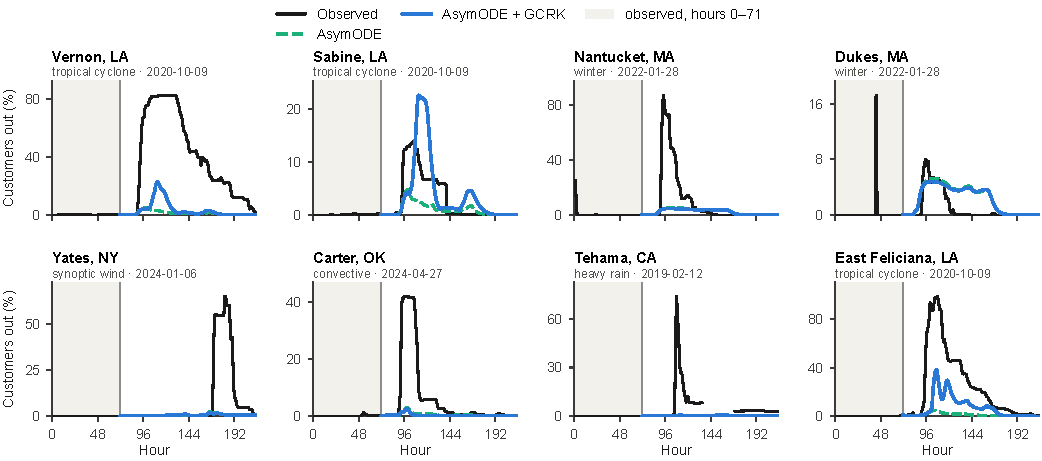
\includegraphics[width=\textwidth]{figures/fig4_trajectories_v1.pdf}
\caption{Outage trajectories for eight held-out counties: the top weather-twin pair of the tropical-cyclone and of the
winter systems (top row), then the county-event with at least 10,000 customers and the largest observed 3-hour peak
among synoptic-wind, convective, heavy-rain and tropical-cyclone systems. Each is forecast by models that never saw
its storm, in one open-loop rollout from hour 71; learned models average five initializations and TimesFM is
zero-shot with the weather as covariates. Shading marks the 72 observed hours.}
\label{fig:traj}
\end{figure*}

\subsection{Model interpretation}
Figure~\ref{fig:geo} compares predicted peaks with the fitting counties' mean descriptors and with each county's own,
in the trained models and without refitting. Own descriptors move a county's predicted peak by \CfGCRKDpeak\ points on
average and by more than half a point in \CfGCRKMoved\ of the county-events; they raise the peaks along the Gulf and
southern Atlantic coasts, lower them across much of the West and move them both ways in the upper Midwest. The design-weighted MSE with own
descriptors is \CfGCRKAll\ relative to the mean descriptors (\CfGCRKTropical\ in tropical and \CfGCRKWinter\ in
winter systems). These changes show the model's sensitivity to its geographic inputs; they do not establish
county-specific vulnerability, and on these data the geography that reaches the kernel does not make its forecasts
more accurate.

\begin{figure*}[t]
\centering
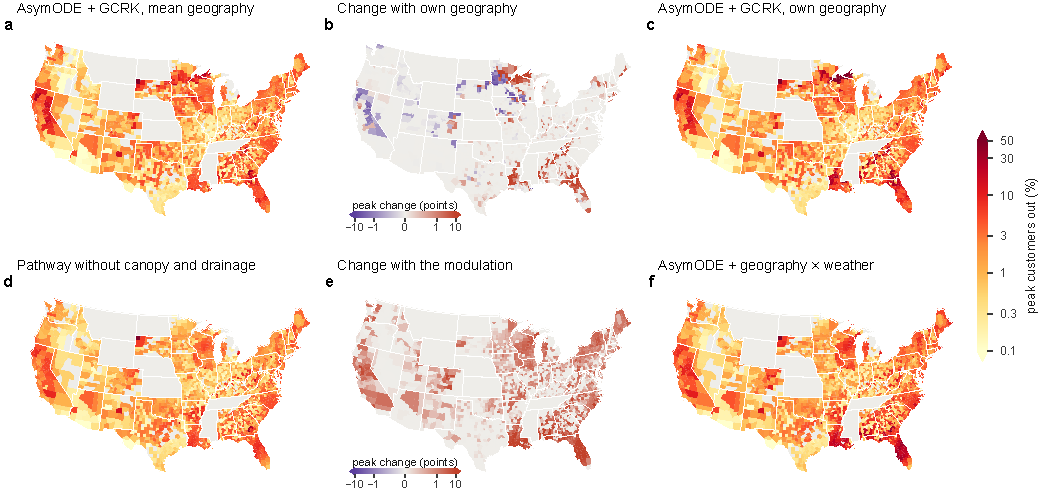
\includegraphics[width=\textwidth]{figures/fig3_geography_v1.pdf}
\caption{Effect of geographic inputs on predicted peak outage fractions in AsymODE + GCRK, per county the largest
over its held-out events. (a) The fitting counties' mean descriptors. (b) The change of the peak when each county's
own descriptors are used, in percentage points (red, an increase). (c) Each county's own descriptors. Panels (a) and
(c) share the colour scale. Nothing is refitted: each trained model is re-run with one input changed.}
\label{fig:geo}
\end{figure*}

\section{Conclusion}
AsymODE combines a bounded population balance with two process-specific neural rates: damage acts on customers still
served, recovery on customers out, so the model supports both initiation from a fully served state and the
restoration of an existing stock. On a designed, event-held-out public benchmark of 81 weather systems of five
regimes, one open-loop forecast per county-event stays close to the all-zero forecast in pooled RMSE, gains where the
outage signal is strong (tropical cyclones, winter storms) and loses in synoptic windstorms and heavy rain. The
geography-conditioned kernel, which lets each county's descriptors shape one temporal response state, does not
improve on the host. Weather twins, neighbouring counties with nearly the same weather and very different outcomes, stay
unresolved, and the largest outages are forecast at a small fraction of their size. Both point to what public data
leave out, namely the location of customers along exposed lines, the condition of the equipment and the course of
the repair, and to where a forecast of this kind has to improve. The sealed confirmatory tranche of 99 systems is
reserved to test the registered claims once they are fixed.

\bibliographystyle{unsrtnat}
\begin{thebibliography}{99}
\bibitem{alpay2020} B.~A. Alpay, D.~Wanik, P.~Watson, D.~Cerrai, G.~Liang, and E.~Anagnostou. Dynamic modeling of power
outages caused by thunderstorms. \emph{Forecasting}, 2(2):151--162, 2020.
\bibitem{brelsford2024} C.~Brelsford et al. A dataset of recorded electricity outages by United States county
2014--2022. \emph{Scientific Data}, 11:271, 2024.
\bibitem{cerrai2019} D.~Cerrai, D.~W. Wanik, M.~A.~E. Bhuiyan, X.~Zhang, J.~Yang, M.~E.~B. Frediani, and E.~N.
Anagnostou. Predicting storm outages through new representations of weather and vegetation. \emph{IEEE Access},
7:29639--29654, 2019.
\bibitem{chen2018} R.~T.~Q. Chen, Y.~Rubanova, J.~Bettencourt, and D.~K. Duvenaud. Neural ordinary differential
equations. In \emph{NeurIPS}, 2018.
\bibitem{das2024} A.~Das, W.~Kong, R.~Sen, and Y.~Zhou. A decoder-only foundation model for time-series forecasting. In
\emph{ICML}, 2024.
\bibitem{dobson2023} I.~Dobson. Models, metrics, and their formulas for typical electric power system resilience
events. \emph{IEEE Transactions on Power Systems}, 38(6):5949--5952, 2023.
\bibitem{hersbach2020} H.~Hersbach et al. The ERA5 global reanalysis. \emph{Quarterly Journal of the Royal
Meteorological Society}, 146:1999--2049, 2020.
\bibitem{kermack1927} W.~O. Kermack and A.~G. McKendrick. A contribution to the mathematical theory of epidemics.
\emph{Proceedings of the Royal Society A}, 115:700--721, 1927.
\bibitem{landsea2013} C.~W. Landsea and J.~L. Franklin. Atlantic hurricane database uncertainty and presentation of a
new database format. \emph{Monthly Weather Review}, 141(10):3576--3592, 2013.
\bibitem{tervo2021} R.~Tervo, I.~L\'ang, A.~Jung, and A.~M\"akel\"a. Predicting power outages caused by extratropical
storms. \emph{Natural Hazards and Earth System Sciences}, 21:607--627, 2021.
\bibitem{zhu2021hotspots} S.~Zhu, A.~Bukharin, L.~Xie, S.~Yang, P.~Keskinocak, and Y.~Xie. Early detection of COVID-19
hotspots using spatio-temporal data. In \emph{ICML Time Series Workshop}, 2021.
\bibitem{zhu2025} S.~Zhu, R.~Yao, Y.~Xie, F.~Qiu, Y.~Qiu, and X.~Wu. Quantifying grid resilience against extreme weather
using large-scale customer power outage data. arXiv:2109.09711v3, 2025.
\end{thebibliography}
\end{document}
